\chapter{The ATLAS experiment}

\textbf{The Inner D}\textit{etector in the hadronic electrode to the tight distribution of the lead to the converted in the tracks and the summary of the electrons are described for the group the group can be simplified in the tracking to the total to the predictions in the tracks as a constants in the distributions are shown}
\vspace{5mm}
\begin{flushright}
--- \textit{autothesis} (\url{https://github.com/mzgubic/autothesis})
\end{flushright}

\thispagestyle{empty}
\newpage

\noindent
The ATLAS experiment is part of the world-leading experimental particle
physics programme hosted by the European Organisation for Nuclear Research
(CERN), designed around the ability to accelerate proton beams to very high
energies and collide them head-on. The protons are accelerated in the Large
Hadron Collider (LHC) and collided at four interaction points
around the LHC ring. The ATLAS detector is built around one of these
interaction points with the purpose of detecting the debris of the
proton-proton collisions. It is designed as a general purpose detector
and is capable of recording data for a wide range of particle physics
searches and measurements.

\section{The Large Hadron Collider}

The Large Hadron Collider is an underground circular proton-proton collider
located in a tunnel under the Swiss-French border near Geneva. It has two
main design goals: to facilitate the collisions at the highest possible
centre-of-mass energy and the highest possible rate. The high rate is
desirable since it allows the study of processes with lower cross-sections, and
the high centre-of-mass energy enables the production of heavy particles as
well as increase the probability of proton-proton interaction.

The protons are obtained by stripping electrons from the hydrogen atoms,
and then pre-accelerated by a sequence of linear and circular accelerators
before entering the main ring. In the main ring the proton beams are
accelerated to 6.5 \TeV and are moving in the opposite directions next to each other
in separate beam pipes. The ring is not perfectly circular but rather consists
of alternating straight sections, which accelerate the protons by passing
them through electromagnetic fields in the superconducting radiofrequency
cavities, and arcs, which bend the proton beam using dipole magnets.
Quadrupole magnets are used close to the interaction points to focus the
beam prior to collisions to increase the collision probability \cite{Brüning:782076}. 

The beams are not a continuous stream of protons but rather a sequence of
proton bunches, each comprising of approximately $10^{11}$ protons. The
bunches cross each other at the interaction point every 25 ns, i.e. a
40 MHz rate. A bunch crossing may result in a collision between
individual protons, and indeed collisions between multiple pairs of
protons are the norm under normal LHC data-taking run conditions.
This effect, known as \pileup, somewhat degrades the quality of
each recorded event and increases the compute time required for the
event reconstruction. However, the majority of interesting physics
involves interactions with high transverse momentum transfer (``hard''),
which are much rarer than the commonplace QCD processes involving
low transverse momentum transfer (``soft''), meaning that the majority
of bunch crossings result in either zero or one hard scatter interactions.

This idea of 

\begin{figure}[h]
  \centering
  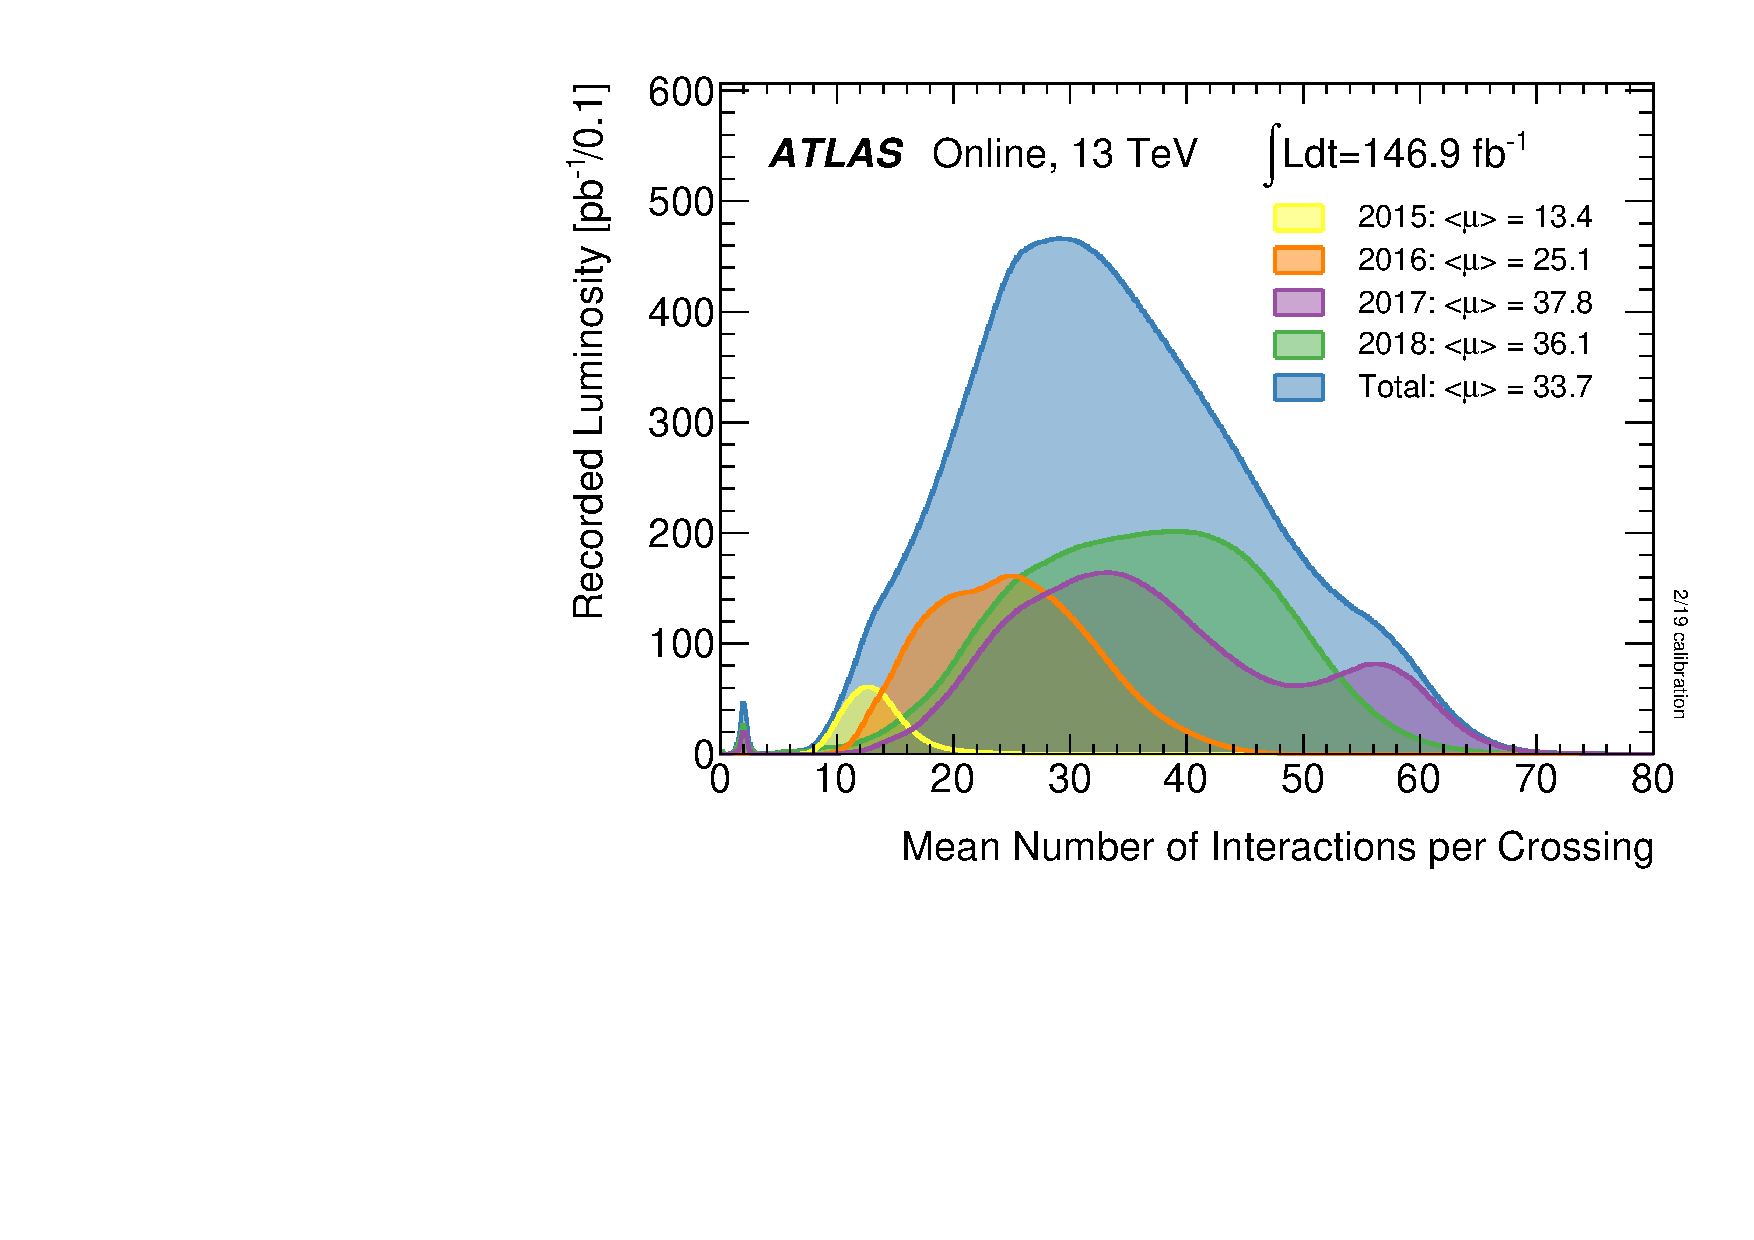
\includegraphics[width=1\textwidth]{figures/experiment/pileup}
  \caption[Mean number of interactions per bunch crossing]{Mean number
  of interactions per bunch crossing. From Ref. \cite{pileup}}
  \label{fig:exp:pileup}
\end{figure}





Each proton beam is accelerated to 6.5 TeV, resulting
in 13 TeV centre-of-mass energy.

\section{Trigger}

\section{Tracking}

\section{Calorimetry}

\section{Muon spectrometry}

\begin{figure}[h]
  \centering
  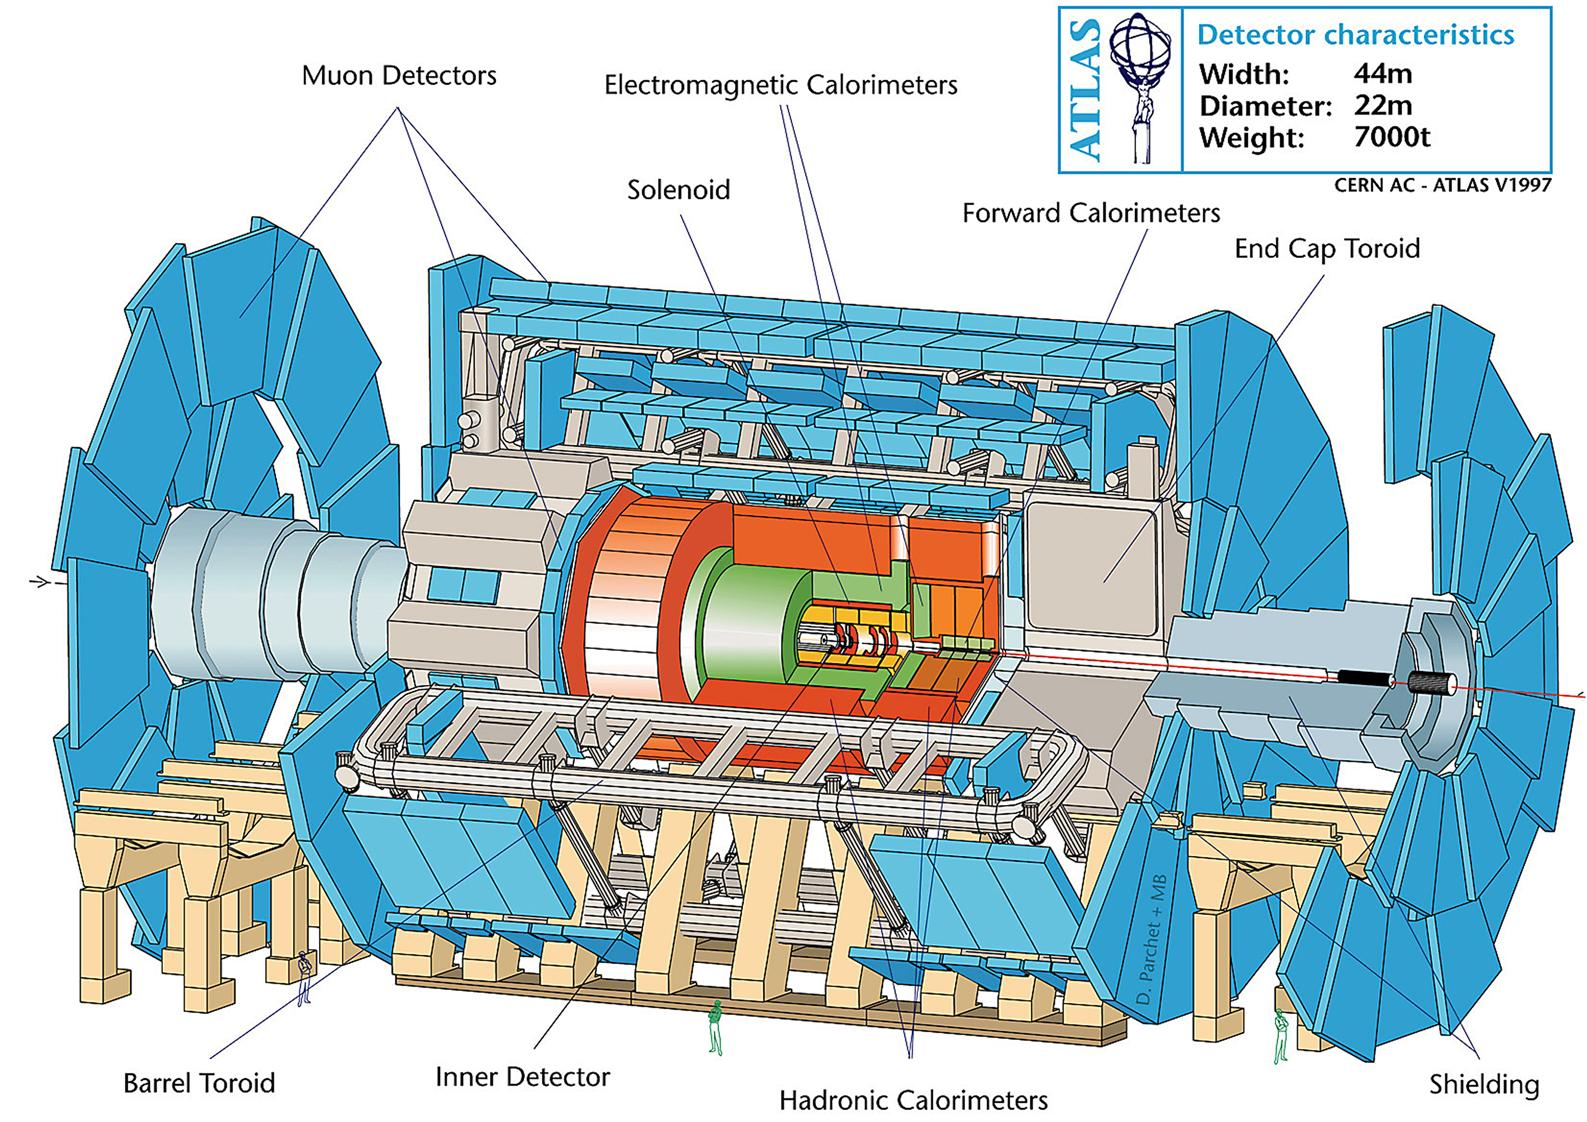
\includegraphics[width=1\textwidth]{figures/experiment/atlas}
  \caption[The ATLAS detector.]{The ATLAS detector. From Ref. \cite{CERN:39038}}
   \label{fig:exp:atlas}
\end{figure}
